%==============================================================================
%====  2.  LINEAR MODELS BASICS  =============================================
%==============================================================================

  %\sampart{B. linear models}\label{chap:linear}
  \sampart{B. linear classification}\label{chap:linear}

    \samsection{0. linear approximations}
      \samquote{
        He had bought a large map representing the sea, \\
        Without the least vestige of land: \\
        And the crew were much pleased when they found it to be \\
        A map they could all understand.
      }{charles dodgson}

%~~~~~~~~~~~~~~~~~~~~~~~~~~~~~~~~~~~~~~~~~~~~~~~~~~~~~~~~~~~~~~~~~~~~~~~~~~~~~~
%~~~~~~~~~~~~~  2.0. featurization  ~~~~~~~~~~~~~~~~~~~~~~~~~~~~~~~~~~~~~~~~~~~

      \sampassage{featurization}  % as an art of
        As in the prologue, we represent our input $x$ as a fixed-length list
        of numbers so that we can treat $x$ with math. 
        There, we
        represented each photograph by $2$ numbers: height and darkness.  We
        could instead have represented each photograph by $784$ numbers, one
        for the brightness at each of the $28\cdot 28=784$ many pixels.  Or by
        $10$ numbers, each measuring the overlap of $x$'s ink with that of
        ``representative'' photos of the digits $0$ through $9$.

        When we choose how to represent $x$ by a list of numbers, %
        we're
        choosing a \textbf{featurization}.  We call each number a ``feature''.
        For example, height and darkness are two features.

        %``height'' and ``darkness'' are \emph{features}: maps $\xX\to \Rr$ used
        %to pre-process $x$s.

        \attnsam{TODO: mention one-hot, etc}
        \attnsam{TODO: mention LOWRANK (sketching; also, for multiregression)}
        %
        There are lots of interesting featurizations, each making different
        patterns easier to learn.\marginnote{%
            \attnsam{data-based featurizations via kernels}
            \attnsam{will soon learn featurizations}
            \attnsam{hand featurization in kaggle and medicine}
        }
        We judge a featurization not in a vacuum but with respect to
        the kinds of patterns we use it to learn. %
        \attnsam{TODO: graphic of separability; and how projection can reduce it}
        Learning usually happens
        more accurately, robustly, and interpretably when our featurization is
        abstract (no irrelevant details) but complete (all relevant details),
        compressed (hard to predict one feature from the others) but accessible
        (easy to compute interesting properties from features).

        Here are three featurizations ideas that might inspire you in
        your own projects.

        \emph{Hardcoded coordinate transforms}.
        %
        \textbf{The bias trick}.\bcirc\marginnote{
            \blarr a.k.a.\ \textbf{projectivization}
        }
        We send
        $x \mapsto (1, x)$, thus increasing dimension by one.
        %\attnsam{TODO: projectivization (say this foreshadows kernel discussion?)}
        %
        \par
        Generalizing the above, we can
        use \textbf{polynomial features}:
        $$
            x \mapsto (x^{\otimes 0}, x^{\otimes 1}, \cdots, x^{\otimes d})
        $$
        By $x^{\otimes d}$, we mean a multiaxis array $a$ with $d$ axes and
        defined (in an example where $d=3$) by
        $$
            a_{42,686,0} = x_{42} x_{686} x_0 \in \Rr
        $$
        Note that this featurization is redundant since permuting $a$'s axes
        doesn't change $a$.
        %
        \par
        \textbf{coordinate transforms} --- e.g.\ arctan.

        \emph{Encoding the discrete}.
        \textbf{one-hot}
        %
        \par
        \textbf{Binning}

        \emph{Data-dependent transforms}.
        %
        \textbf{Quantilization}
        %
        \par
        \textbf{Landmarks}

        %In the exercise at the end of the passage on ``meeting the data'', we
        %dreamed up other ``features'' (besides \emph{height} and
        %\emph{darkness}) that might help to distinguish ${\red{9}}$s
        %from ${\cya{1}}$s.
        %%
        %Maybe we thought of \emph{width}.  Or of whether the ink surrounds a
        %\emph{hole}, as in a ${\red{9}}$.  Or of a photo's \emph{topheaviness}:
        %is its top half darker than its bottom half?  We might have chosen a
        %`canonical' photo of each of the digits in order to consider how a
        %given photo's ink \emph{overlaps} with those canonical photos'.
        %%
        %These are just some of very many good ideas.

        %Let's crudely define a photo as having a \emph{hole} at location
        %$(r,c)$ when, for each quadrant around $(r, c)$, location
        %$(r,c)$ is strictly brighter than a location in that quadrant.  A
        %photo's \emph{holiness} is the fraction of its pixels that are holes.

        %And let's define the \emph{overlap} between two photos as the fraction
        %of their pixels that are both above or both below $0.5$ in darkness.

        %\begin{lstlisting}[language=Python, basicstyle=\footnotesize\ttfamily]
        %  SIDE = 28
        %  def darkness(x):
        %    return np.mean(np.mean(x))
        %  def height(x):
        %    return np.std([row for col in range(SIDE)
        %                       for row in range(SIDE)
        %                       if 0.5 < x[row][col]  ])/(SIDE/2.0)
        %  def width(x):
        %    return np.std([row for col in range(SIDE)
        %                       for row in range(SIDE)
        %                       if 0.5 < x[row][col]  ])/(SIDE/2.0)
        %  def holiness(x):
        %    return np.mean([1 if (np.max(x[:row,:col]) > x[row,col] and
        %                          np.max(x[:row,col:]) > x[row,col] and
        %                          np.max(x[row:,:col]) > x[row,col] and
        %                          np.max(x[row:,col:]) > x[row,col]    ) else 0
        %                      for col in range(1,SIDE-1)
        %                      for row in range(1,SIDE-1)                       ])
        %  def topheaviness(x):
        %    return (np.mean(x[:int(SIDE/2)])-np.mean(x[int(SIDE/2):]) + 1.0)/2
        %  #def overlap_one(x):
        %  #  return np.sum()
        %  #def overlap_nine(x):
        %\end{lstlisting}
        %We normalized all features so that they output values in $[0.0,1.0]$.

        %\par\noindent
        %\attn{Exercise:} {How might our ${\red{9}}$ vs ${\cya{1}}$ model fail
        %to generalize to photos of unevenly lit paper?  Photos of lined paper?
        %Of chalk on slate?  Of $7$-segment digital displays?
        %\par\noindent
        %\attn{Exercise:} {How might they fail for classifying $3$ vs $8$?}
%~~~~~~~~~~~~~~~~~~~~~~~~~~~~~~~~~~~~~~~~~~~~~~~~~~~~~~~~~~~~~~~~~~~~~~~~~~~~~~
%~~~~~~~~~~~~~  2.1. geometry of feature-space  ~~~~~~~~~~~~~~~~~~~~~~~~~~~~~~~

      \sampassage{geometry of feature-space} % pictures!
        Say we've decided on a \textbf{featurization} of our input
        data $x$.
        %$$
        %  f_{a,b}(x) = ~0 \text{~~if~~} a\cdot \text{width}(x) + b\cdot\text{darkness}(x) < 0 \text{~~else~~} 1
        %$$
        \begin{marginfigure}
          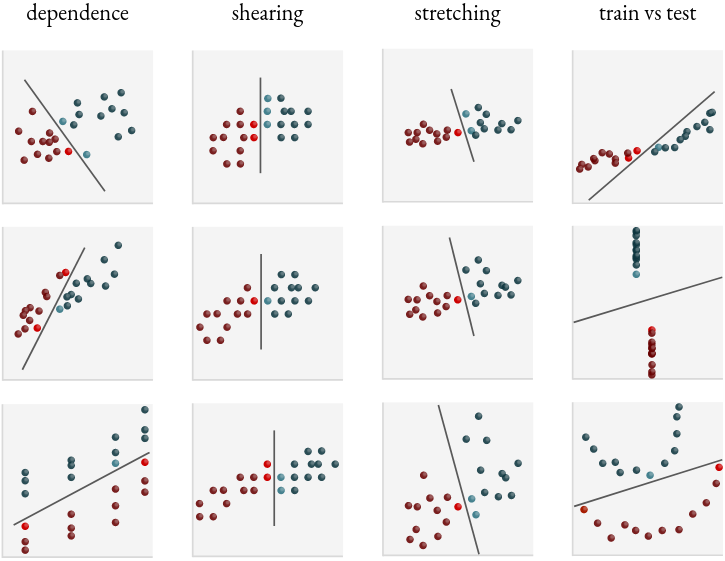
\includegraphics[width=\textwidth]{feature-space-phenomena}
        \end{marginfigure}

        % dependence
        Just because two features both correlate with a positive label ($y=+1$)
        doesn't mean both features will have positive weights.  In other words,
        it could be that the \emph{blah}-feature correlates with $y=+1$ in the
        training set and yet, according to the best hypothesis for that
        training set, the bigger a fresh input's blah feature is, the
        \emph{less} likely its label is to be $+1$, all else being equal.  That
        last phrase ``all else being equal'' is crucial, since it refers to our
        choice of coordinates.
        %
        \attnsam{Illustrate `averaging' of good features vs `correction' of one
        feature by another (how much a feature correlates with error)}
        %
        In fact, t This is the difference between \emph{independence} and
        \emph{conditional independence}.

        % shearing
        Shearing two features together --- e.g.\ measuring
        cooktime-plus-preptime together with cooktime rather than preptime
        together with cooktime --- can impact the decision boundary.
        %
        Intuitively, the more stretched out a feature axis is, the more the
        learned hypothesis will rely on that feature.

        % stretching
        Stretching a single feature --- for instance, measuring it in
        centimeters instead of meters --- can impact the decision boundary
        as well.  Intuitively, the more stretched out a feature axis is,
        the more the learned hypothesis will rely on that feature.

        % train vs test
        Note that

        %Caution: a feature $A(\sfx)$ that is statistically independent from
        %$\sfy$ may still be relevant for predicting $\sfy$.\marginnote{%
        %  Example.  Consider the uniform distribution on the four corners of a
        %  tetrahedron embedded within the corners of a cube \attnsam{TODO:
        %  graphic}.  The three spatial coordinates give three bit-valued random
        %  variables.  Any two of these variables are independent.  But the
        %  three together are dependent.
        %  \attnsam{TODO: also do a decision boundary (simpsons style) graph
        %  illustrating this phenomenon}
        %}
        %For example, if
        %$A, B$ are two features, it is possible that $A(\sfx), \sfy$ are
        %independent and that $B(\sfx), \sfy$ are independent and yet
        %$A(\sfx),B(\sfx), \sfy$ are \emph{dependent}!

        \attnsam{TODO: example featurization (e.g. MNIST again?)}

%~~~~~~~~~~~~~~~~~~~~~~~~~~~~~~~~~~~~~~~~~~~~~~~~~~~~~~~~~~~~~~~~~~~~~~~~~~~~~~
%~~~~~~~~~~~~~  2.2. richer outputs  ~~~~~~~~~~~~~~~~~~~~~~~~~~~~~~~~~~~~~~~~~~

      %\sampassage{richer outputs: larger $\yY$}
      \sampassage{more classes and beyond}
        We've learned how to construct a set $\hH$ of candidate patterns
        $$
          f_{\vec w}(\vec x) = \text{step}(\vec w\cdot \vec x)
        $$
        that map (a featurization of) a prompt $\vec x$ to a binary answer
        $y=0$ or $y=1$.

        What if we're interested in predicting a richer kind of $y$?  For
        example, maybe there are $k$ many possible values for $y$ instead of
        just $2$.  Or maybe there are infinitely many possible values --- say,
        if $y$ is a real number or a length-$k$ list of real numbers.  Or maybe
        we want the added nuance of predicting probabilities, so that $f$ might
        output ``19\% chance of label $y=0$ and 80\% chance of label $y=1$ and
        1\% chance of label $y=2$''
        instead of just ``$y=1$''.

        I'll write formulas and then explain.
        \begin{align*}
            \text{multi-class hard classification}\quad&
            f_{(\vec w_i : 0\leq i < k)}(\vec x) = \text{argmax}_i(\vec w_i\cdot \vec x : 0\leq i<k)
        \\
            \text{multi-output regression}\quad&
            f_{(\vec w_i  : 0\leq i < k)}(\vec x) = (\vec w_i \cdot \vec x : 0\leq i < k)
        \\
            \text{multi-class soft classification}\quad&
            f_{(\vec w_i  : 0\leq i < k)}(\vec x) = \text{normalize}(\exp(\vec w_i \cdot \vec x) : 0\leq i < k)
        \end{align*}

        A key ideas here is \emph{symmetry between classes}.  Previously, we
        interpreted positive decision function values as meaning one class and
        negative values as meaning the other.  This is asymmetrical --- why
        should one class count as positive?! --- and does not immediately
        generalize to multiple classes.
        %
        Instead, let's do two-class classification by producing \emph{two}
        values: the degree to which a point is of one class
            and the degree to which a point is of the other class.
        Then we'll classify according to which value is \emph{greater}.
        This is redundant because we could add $+42$ to both values and get the
        same answer for all inputs.  Redundancy is often the cost of symmetry.

        More generally, if we have three classes \emph{ostrich}, \emph{emu},
        and \emph{roc}, then we compute three linear functions representing
        \emph{ostrich-ness}, \emph{emu-osity}, and \emph{roc-iness}.  And we
        return whichever class has a greatest value.  This explains the
        \emph{multi-class hard classification}.

        For \emph{multi-output regression}, let's just skip the argmax.

        For \emph{multi-output soft classification}, we want to report
        probabilities instead of general real-valued scores.  Probabilities
        ought to be non-negative and ought to sum to one.  A nice way to turn
        general numbers to non-negative (in fact, positive) ones is to apply
        $\exp$.  A nice way to get positive numbers to sum to $1$ is to divide
        by their sum.  This leads us to \textbf{softmax}:
        $$
          \text{softmax}(\omega_k ~:~ 0\leq k<K) = \left(\frac{\exp(\omega_k)}{\sum_{k^\prime} \exp(\omega_{k^\prime})} ~:~ 0\leq k<K\right)
        $$

        %\attnsam{TODO: interpret}
        \attnsam{TODO: show pictures of 3 classes, 4 classes (e.g. digits 0,1,8,9)}
        %\attnsam{TODO: discuss measures of goodness!}
        \attnsam{TODO: talk about structured (trees/sequences/etc) output!}

%~~~~~~~~~~~~~~~~~~~~~~~~~~~~~~~~~~~~~~~~~~~~~~~~~~~~~~~~~~~~~~~~~~~~~~~~~~~~~~
%~~~~~~~~~~~~~  2.3. richer outputs  ~~~~~~~~~~~~~~~~~~~~~~~~~~~~~~~~~~~~~~~~~~

      \sampassage{visualizing high dimensional spaces}
        \attnsam{FILL IN}


